\documentclass{beamer}

\usepackage{graphicx}
\usetheme{Szeged}
\usecolortheme{beaver}

\author{Anne Wanningen \and Xeryus Stokkel}
\title[Week 4]{Introduction to Computer Graphics raytracer week 4}

\begin{document}

\maketitle

\section{Results}
\begin{frame}
	\begin{figure}
		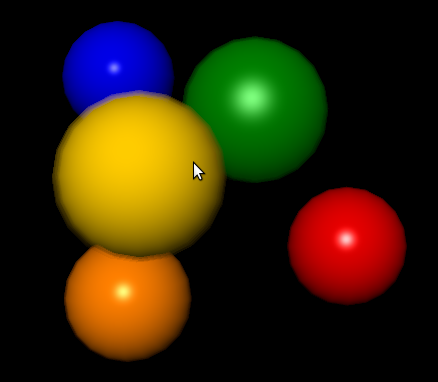
\includegraphics[width=\textwidth]{result.png}
	\end{figure}
\end{frame}

\section{Depth of Field}
\begin{frame}
	\begin{columns}[T]
		\begin{column}{.5\textwidth}
			\begin{figure}
				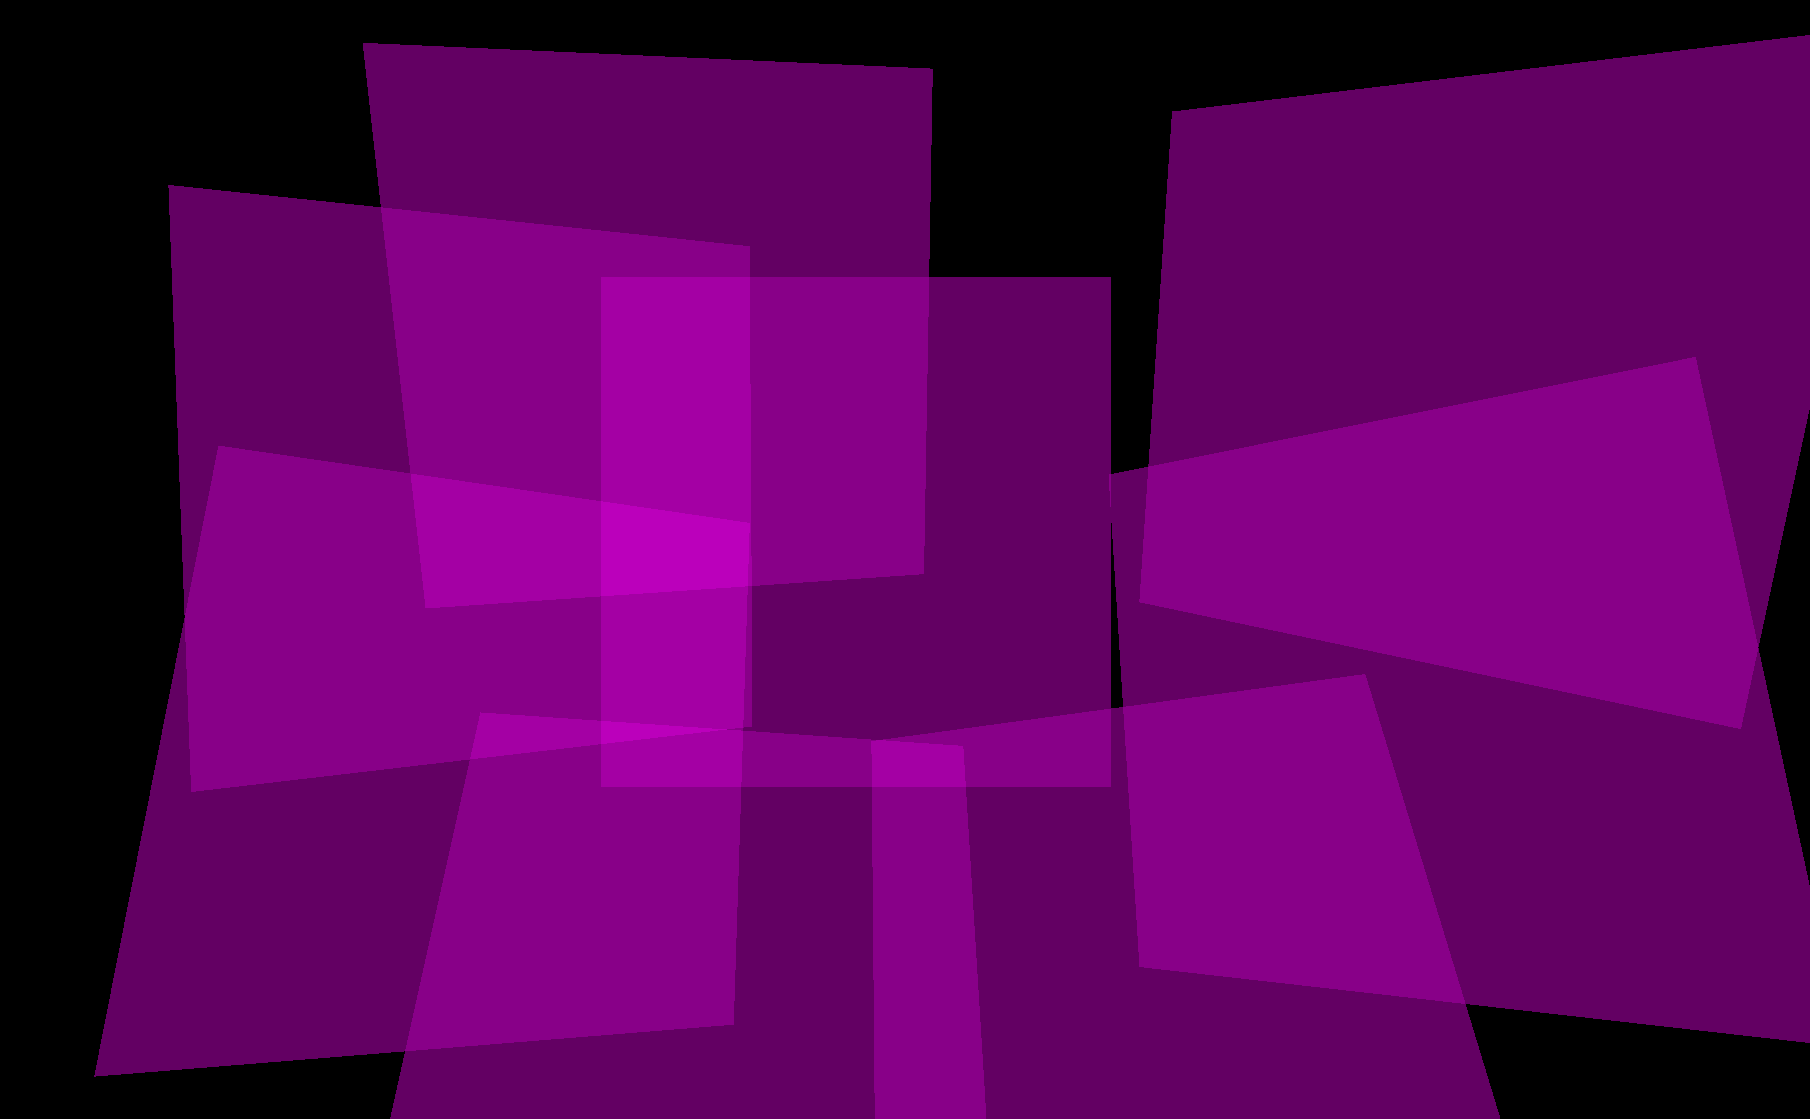
\includegraphics[width=\textwidth]{blurryCubes.png}
			\end{figure}
		\end{column}
		\begin{column}{.5\textwidth}
			\begin{figure}
				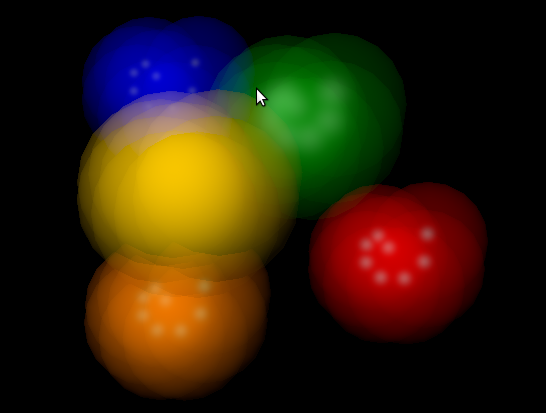
\includegraphics[width=\textwidth]{blurryBalls.png}
			\end{figure}
		\end{column}
	\end{columns}
\end{frame}


\end{document}
